\documentclass[DM,authoryear,toc]{lsstdoc}
\input{meta}
\graphicspath{{./}{figures/}}
\usepackage{amsmath}
% Package imports go here.

% Local commands go here.

%If you want glossaries
%\input{aglossary.tex}
%\makeglossaries

\title{Effects of Persistence and E2V Sensors using DC2 Data}

% Optional subtitle
% \setDocSubtitle{A subtitle}

\author{%
John Banovetz,
Yousuke Utsumi,
Colin Slater
}

\setDocRef{DMTN-276}
\setDocUpstreamLocation{\url{https://github.com/lsst-dm/dmtn-276}}

\date{\vcsDate}

% Optional: name of the document's curator
% \setDocCurator{The Curator of this Document}

\setDocAbstract{%
In this technote, I describe the measurements and characterization of the persistence effect with the E2V sensors. 
I will also describe the process that I used to evaluate the effects persistence would have on the LSST survey. 
For this, I took persistence characterization values from electro-optical testing and modified raw DC2 images to include this model of persistence. 
I then ran the raw images through the DRP and analyzed the results. 
I found that the persistence adds a possibly non-negligible amount of flux to faint sources and can affect a significant amount of pixels. 
}

% Change history defined here.
% Order: oldest first.
% Fields: VERSION, DATE, DESCRIPTION, OWNER NAME.
% See LPM-51 for version number policy.
\setDocChangeRecord{%
  \addtohist{1}{YYYY-MM-DD}{Unreleased.}{John Banovetz}
}


\begin{document}

% Create the title page.
\maketitle
% Frequently for a technote we do not want a title page  uncomment this to remove the title page and changelog.
% use \mkshorttitle to remove the extra pages

% ADD CONTENT HERE
% You can also use the \input command to include several content files.

\section{Electro-optical Measured Persistence}
\subsection{Definition and Run 5 Measurements}

\begin{figure*}[!htp]
  \centering
  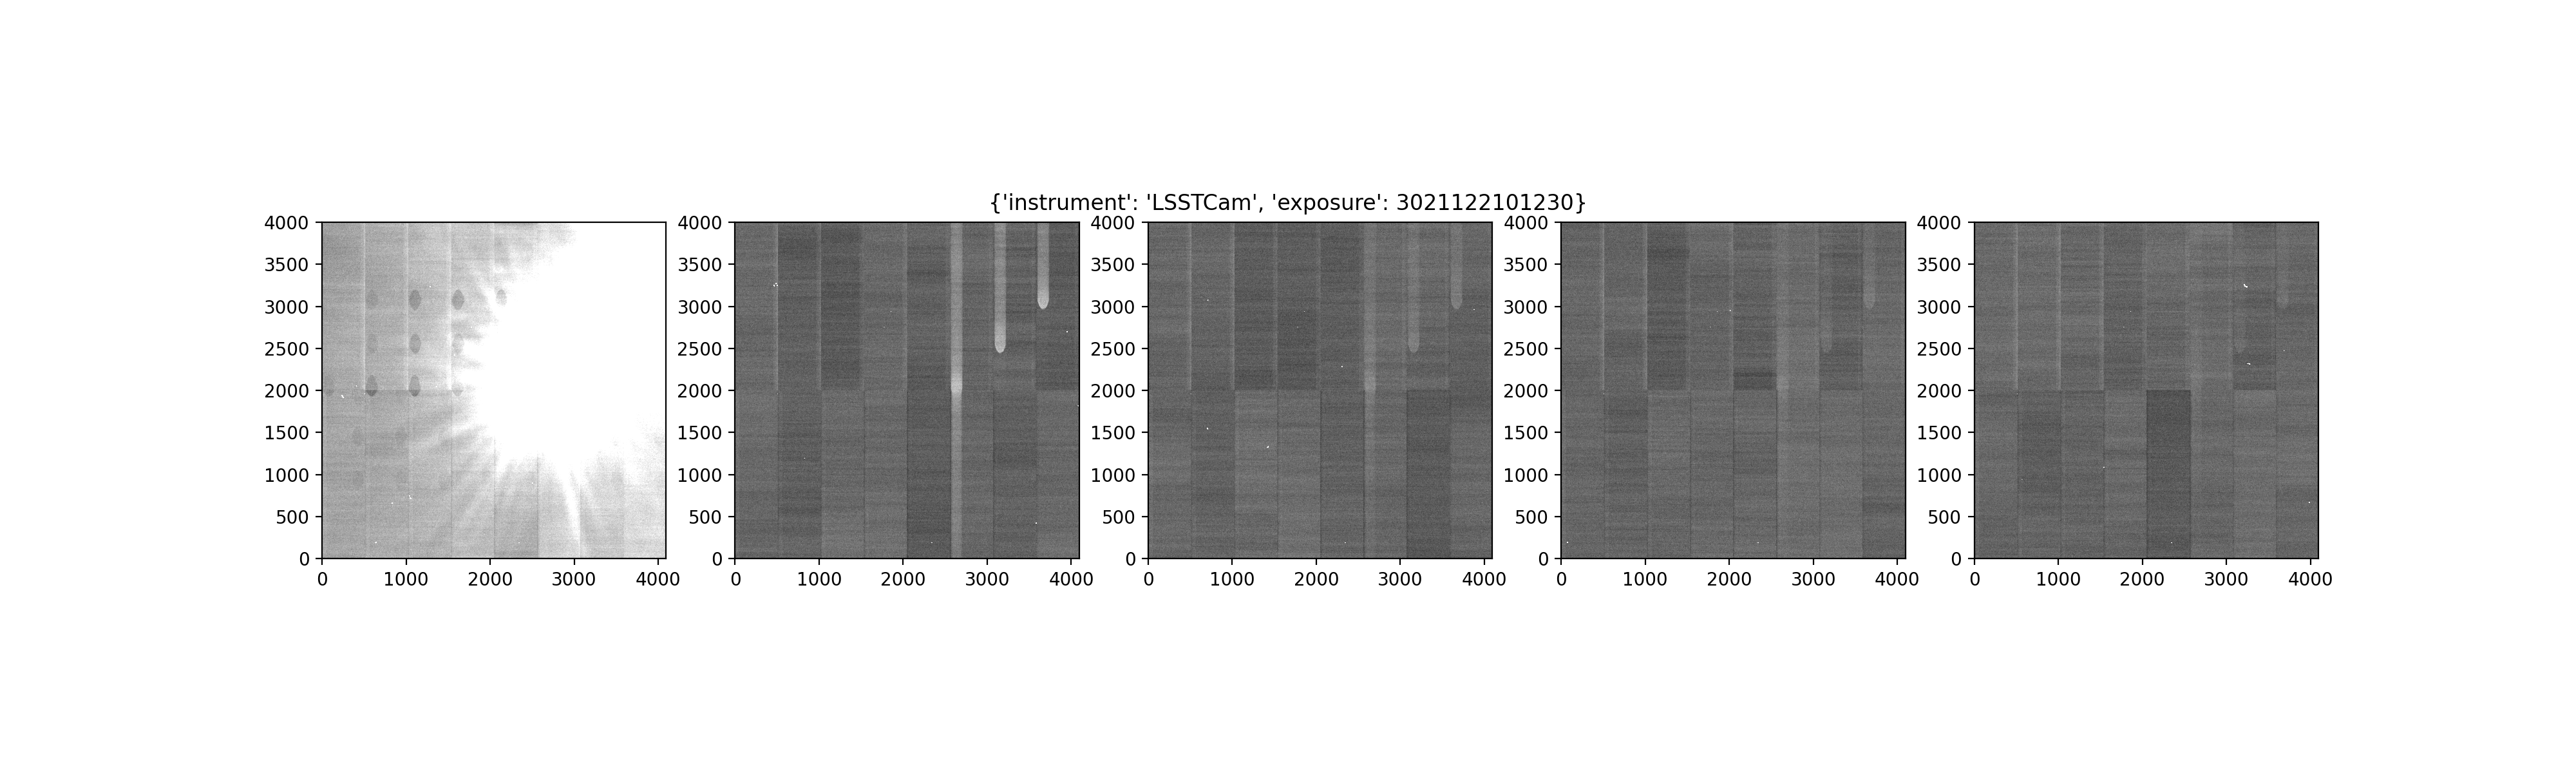
\includegraphics[width=0.95\textwidth, angle=0]{Run_5_persistence_ex.png}
  \caption{
  Example of peristence in Run 5 data. 
  This figure shows the initial flash on the left most image (dataId shown as the title) and the subsquent darks images going from left to right.
  This particular flash has one of the three spots inbetween two amplifiers and you can see the trail starting at the spots and going all the way to the readout of each amplifier.
  }\label{fig:ex_persistence_Run5}
\end{figure*}



Persistence is a sensor level effect where charge gets trapped from one image and `persists' into the next and some fraction of the original charge. 
Figure \ref{fig:ex_persistence_Run5} shows an example of this from Run 5 data where saturated spot persists into subsequent dark images. 
Persistence for LSSTCam was first found in Run 5 of electro-optical (EO) testing at SLAC from crosstalk measurements. 
Further investigation found that this effect only affected E2V sensors. 
% This persistence was found to have an average signal after the flash of 6 ADU and had a decay constant of 37 seconds. 
It was also foud that the persistence only went away with integration time as no persistence was shown in biases. 
One of the unique features of this persistence is the persistence trail. 
Not only do the saturated pixels have an increased signal, but so do all the pixels leading to the end of the amplifier in the parallel direction.

\subsection{Run 6 Measurements}
Following this discovery in Run 5, we tested and characterized the persistence further in Run 6a and 6b. 
This included using both a flat illumnination to induce persistence as well as utilizing a pinhole filter to create saturated spots to measure the persistence.

\subsubsection{Flat Induced Persistence}
\begin{figure*}[!htp]
  \centering
  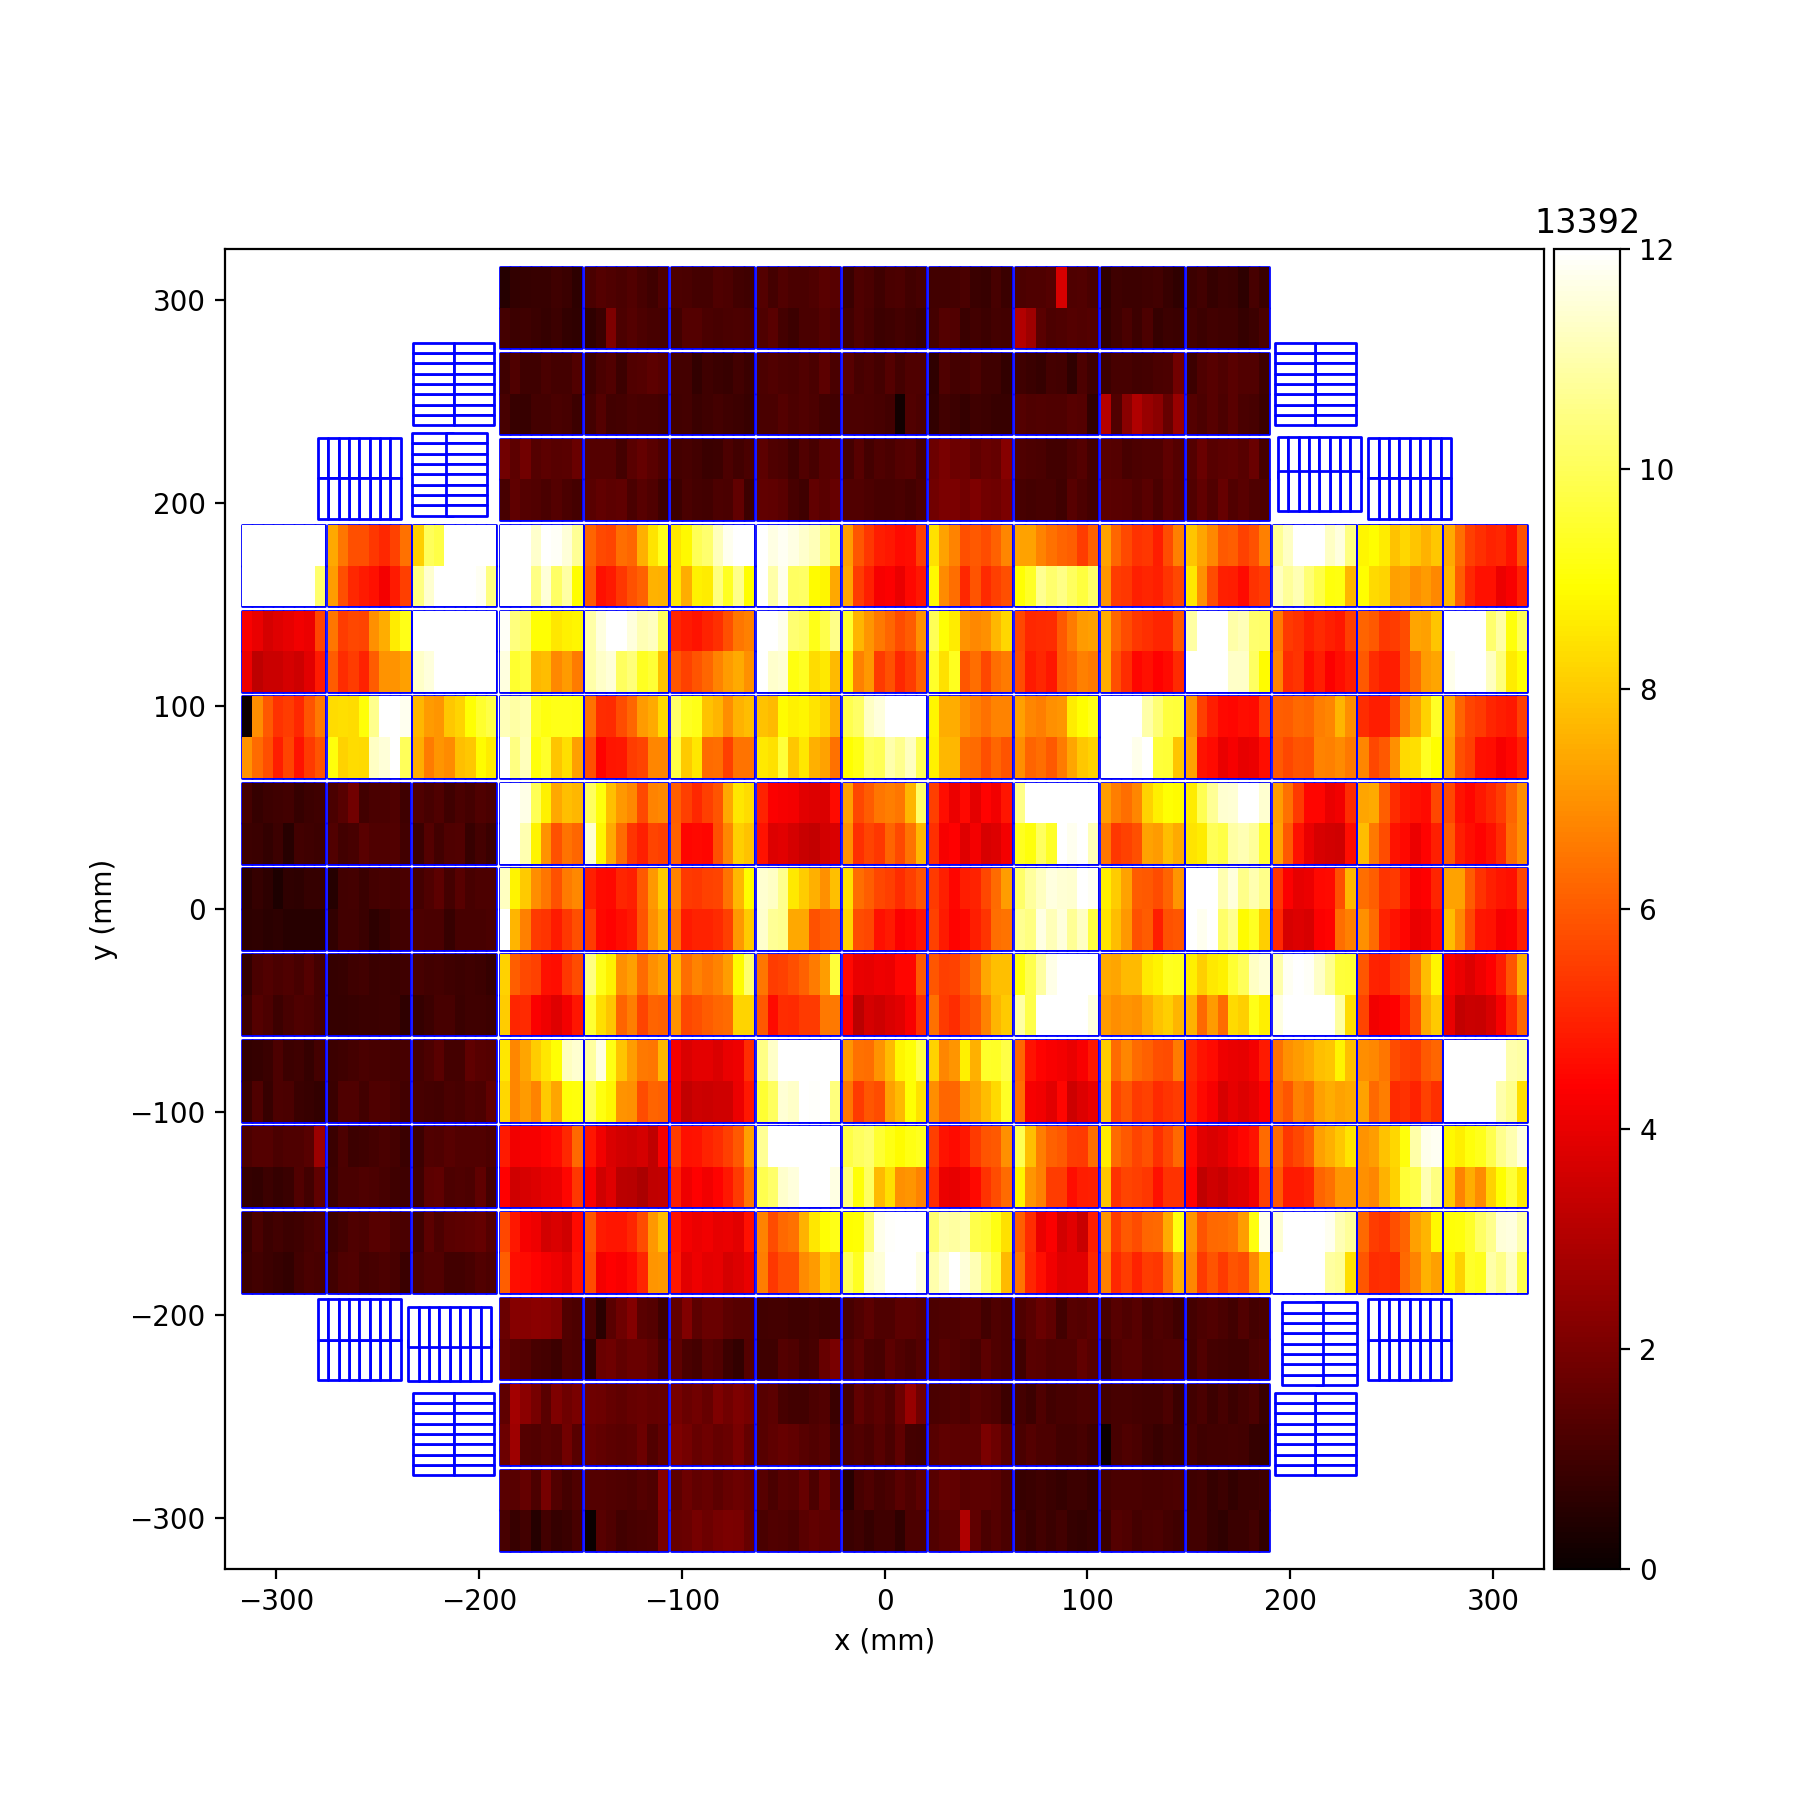
\includegraphics[width=0.45\textwidth, angle=0]{Run_13392_Persistence.png}
  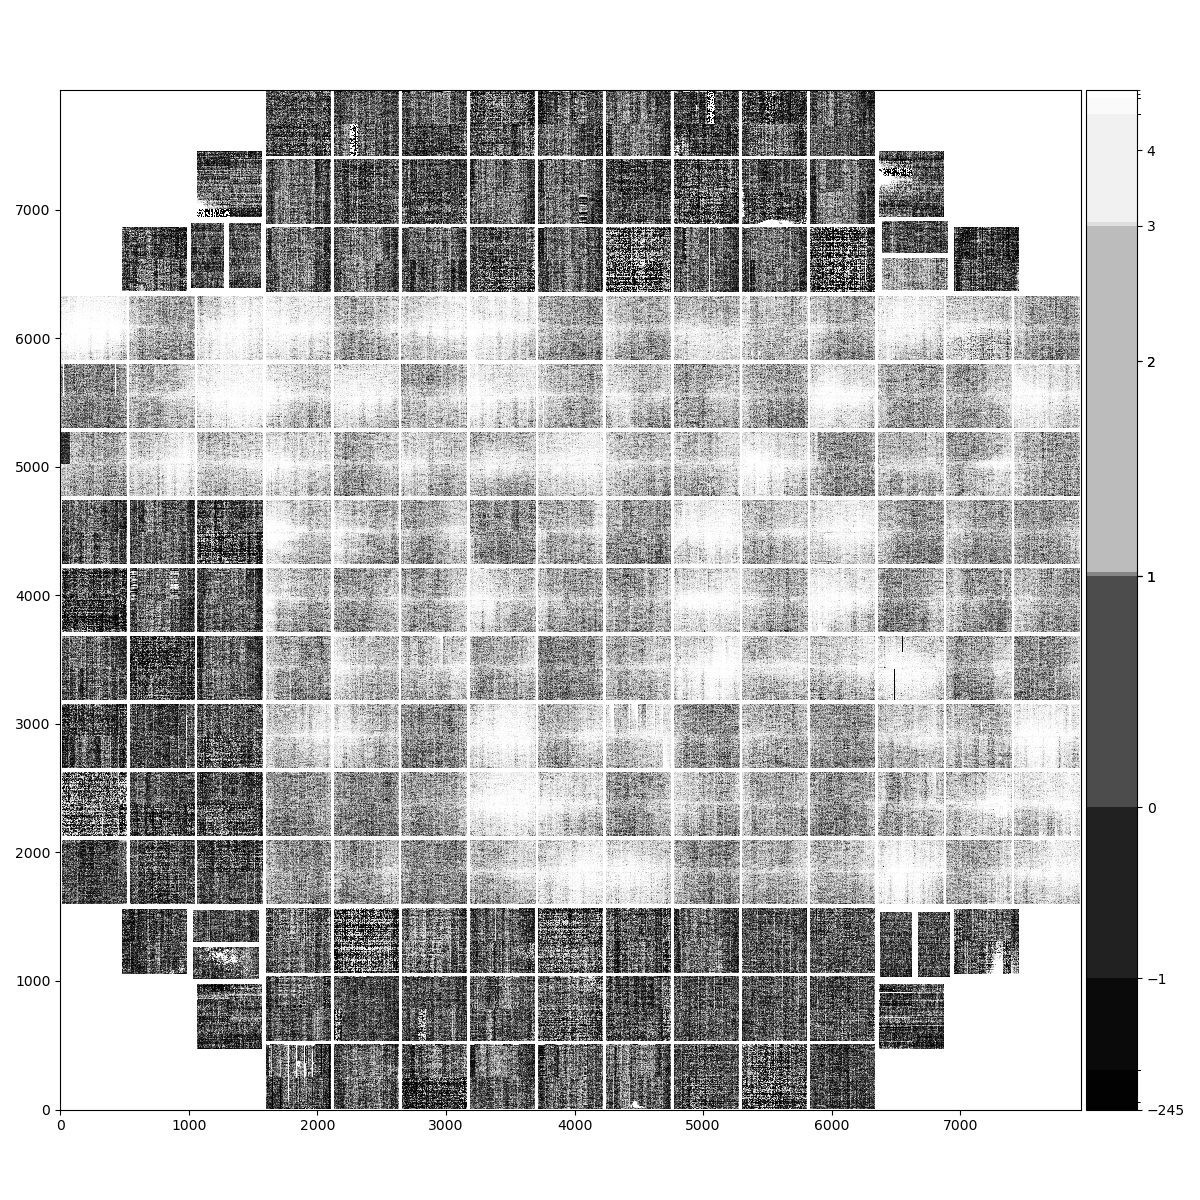
\includegraphics[width=0.45\textwidth, angle=0]{Persistence_Flat_Example.png}
  \caption{
  Full focal plane images of the counts in the first dark image after a bright exposure for run 13392.
  The left shows the amplifier level average for all science sensors of the subsequent dark.
  The right shows a binned image of the dark image from RubinTV\@.
  % This particular flash has one of the three spots inbetween two amplifiers and you can see the trail starting at the spots and going all the way to the readout of each amplifier.
  }\label{fig:Flat_Induced}
\end{figure*}

Flat illuminated persistence measurements were taken during B and C protocol runs.
The procedure for these measurements were to take a incredibly bright (3~4 times full well) flat followed by 15 second dark images.
These images are then run through both $\texttt{cp_pipe}$ and $\texttt{eo_pipe}$.
This is to induce the persistence, determine the level and then track its decay.
Unfortunately this method does not allow us to measure the trail caused by the the persistence as all the pixels are saturated.

\begin{figure*}[!htp]
  \centering
  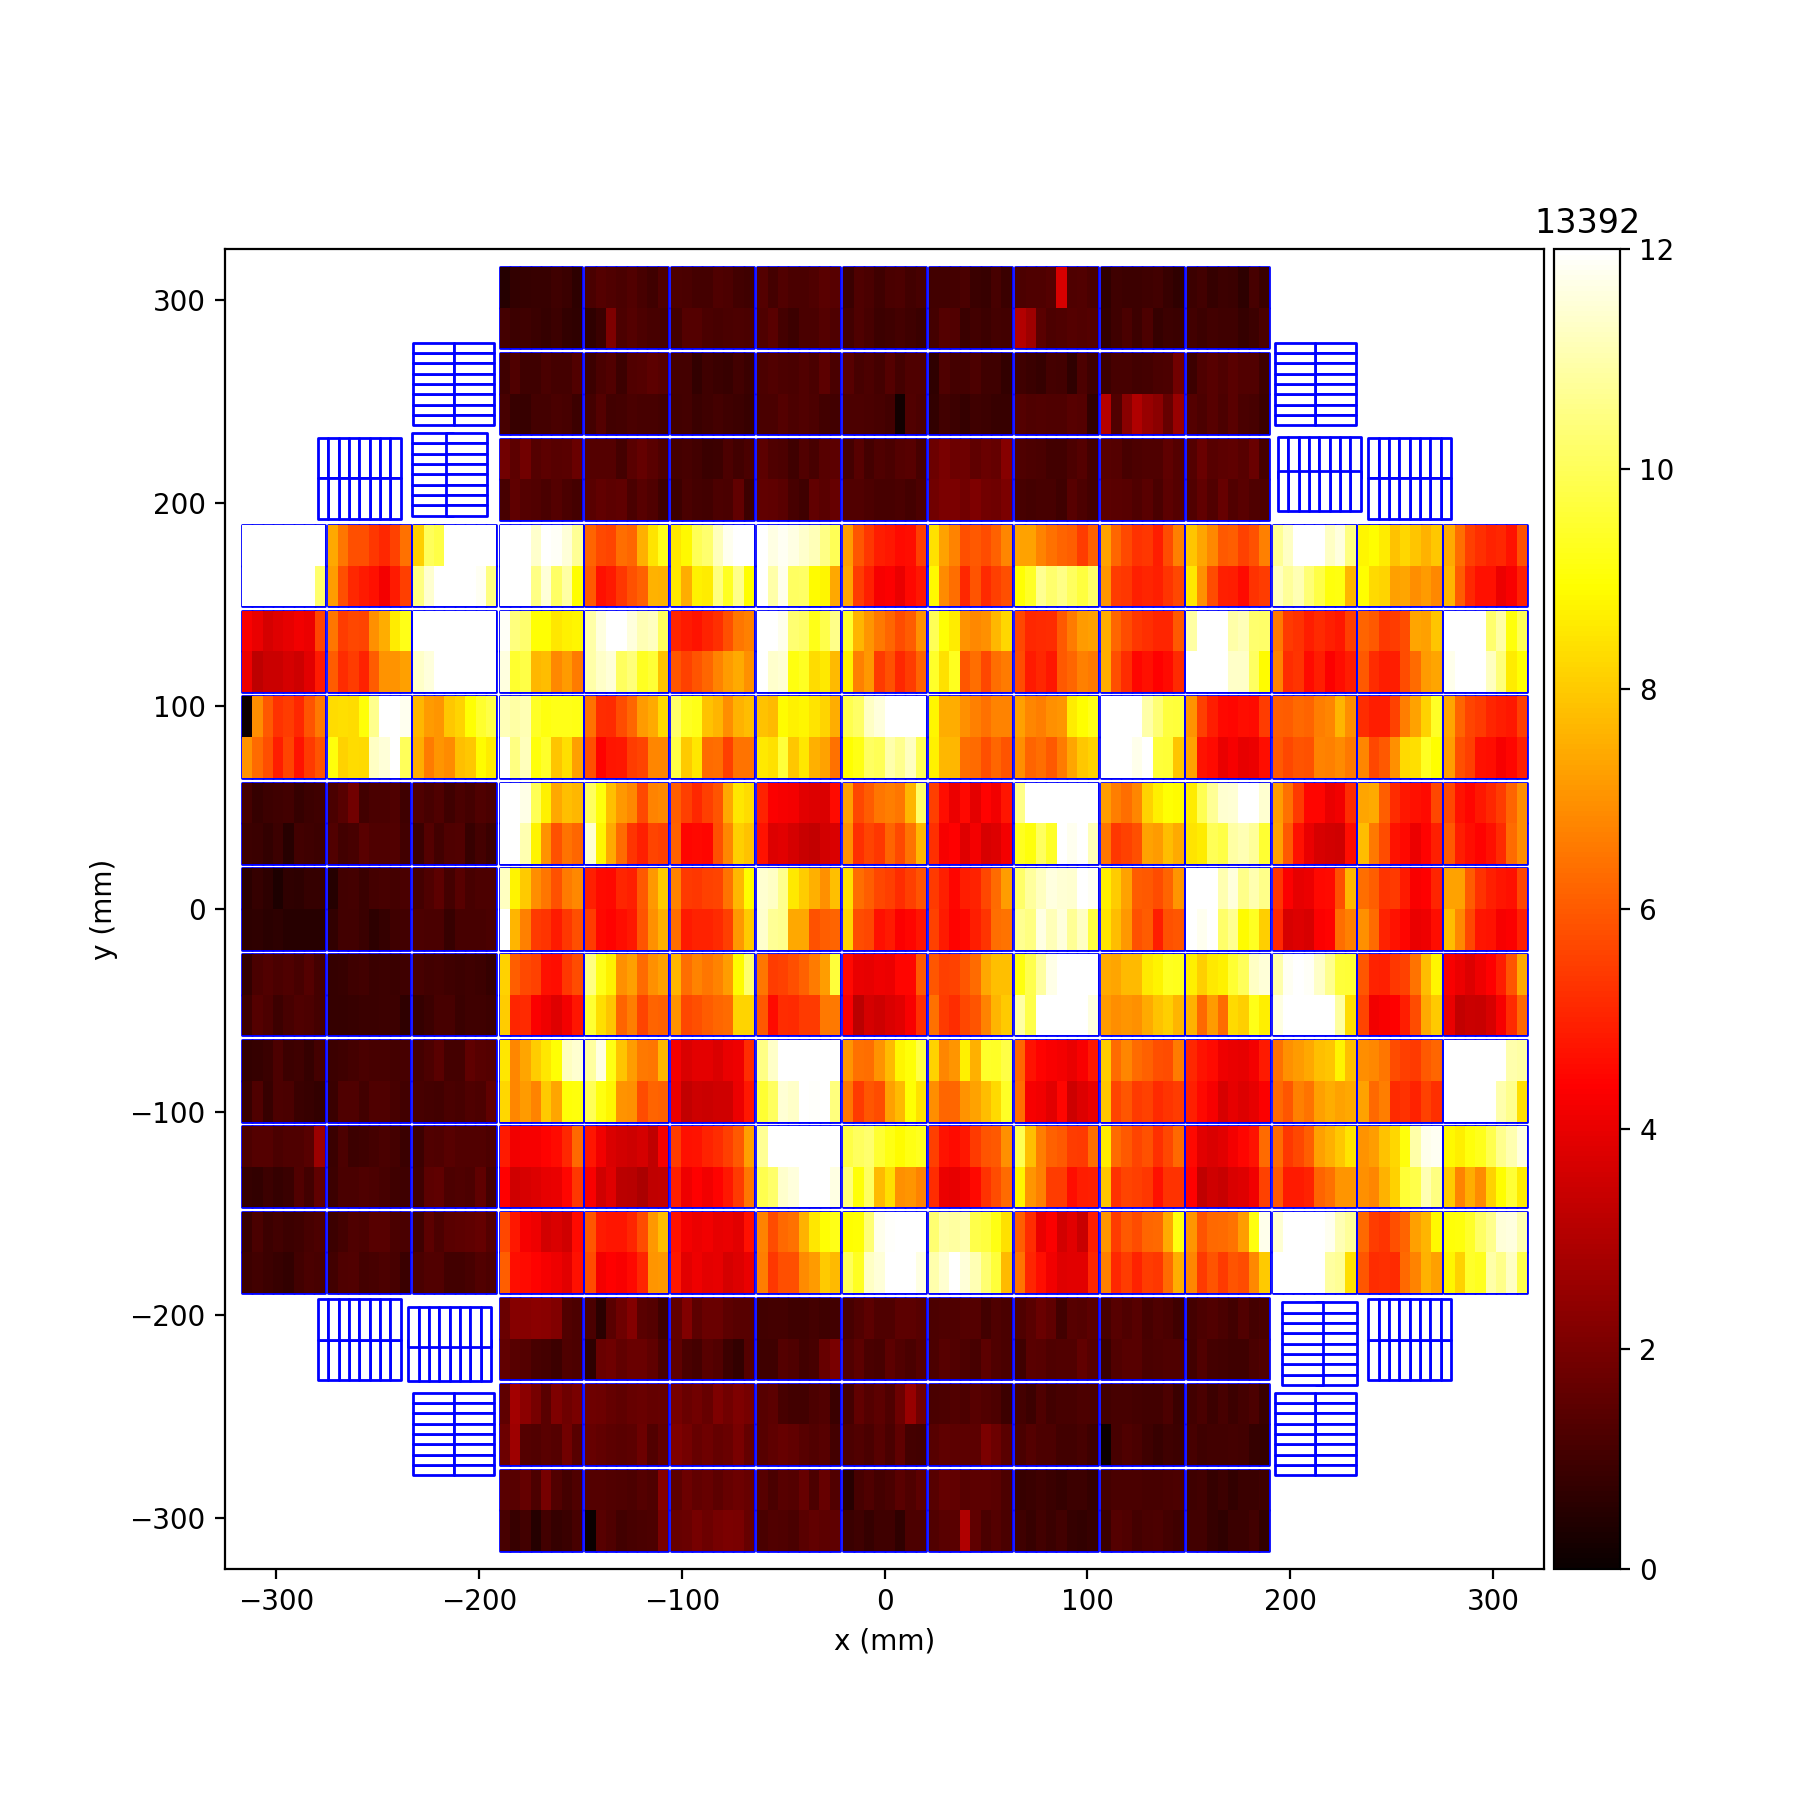
\includegraphics[width=0.45\textwidth, angle=0]{Run_13392_Persistence.png}
  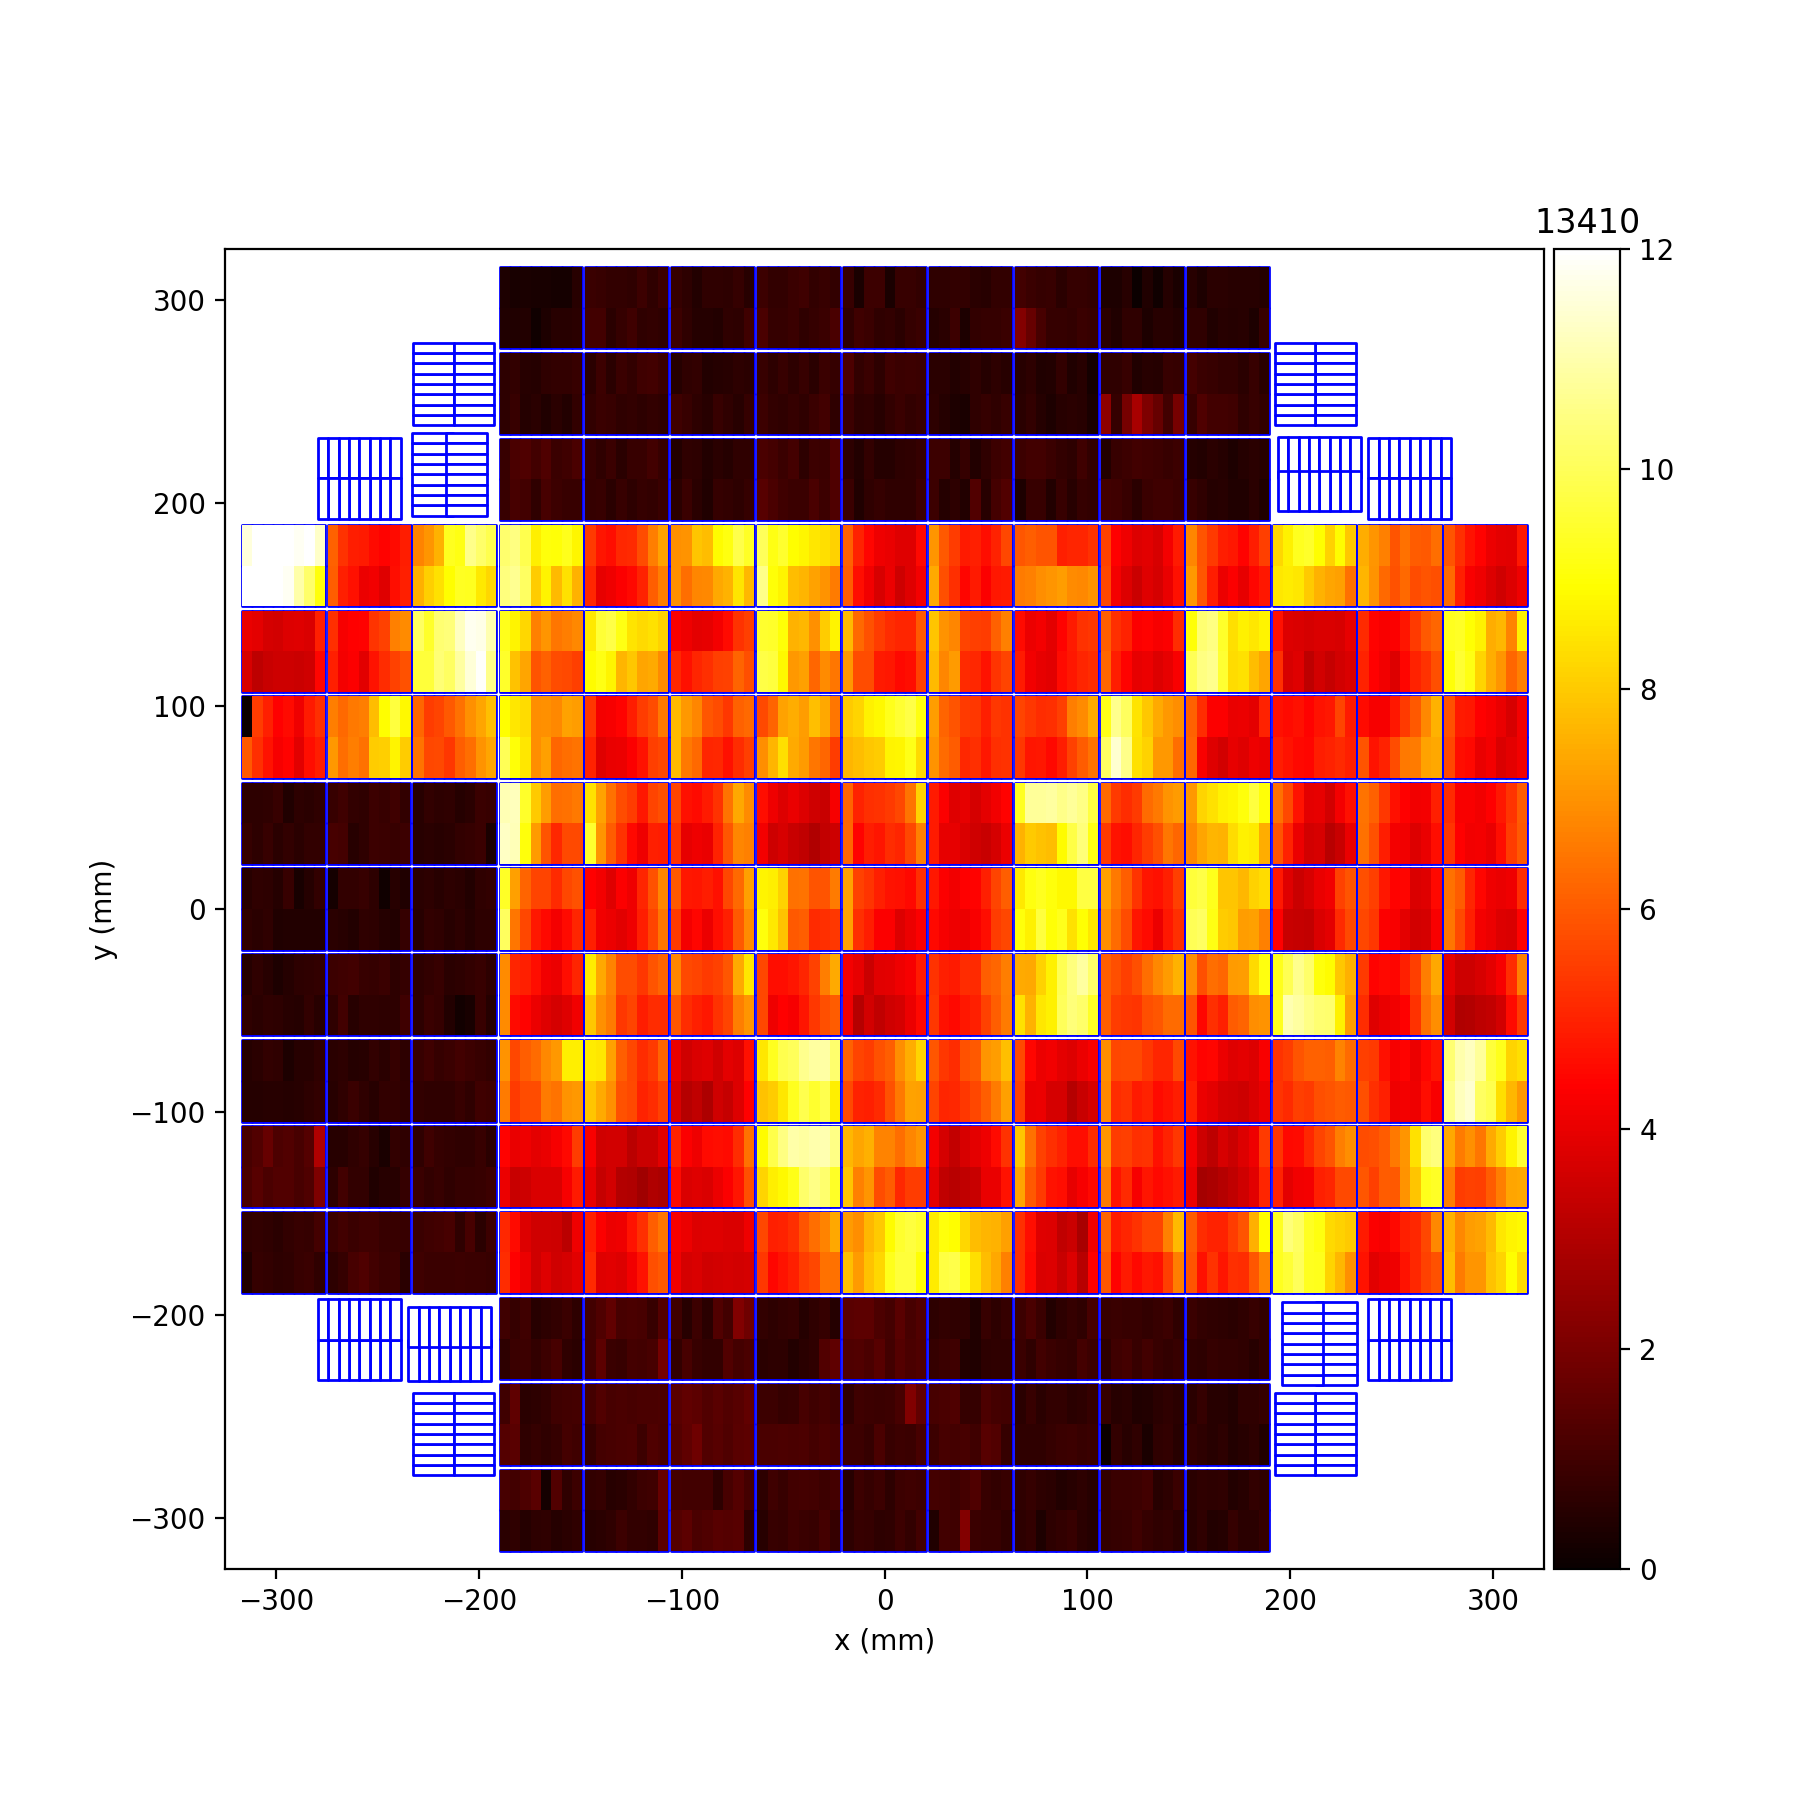
\includegraphics[width=0.45\textwidth, angle=0]{Run_13410_Persistence_Lower.png}
  \caption{
  Full Focal plane images with amplifier level resoltuion comparing a subsequent dark image with nomial parallel clock swing voltages (left; Run 13392) 
  and one with a slightly higher parallel clock swing voltage (right; Run 13410).
  % This particular flash has one of the three spots inbetween two amplifiers and you can see the trail starting at the spots and going all the way to the readout of each amplifier.
  }\label{fig:Flat_Induced_Comparison}
\end{figure*}

One of the concerning discoveries with these measurements were the level of persistence was reaching 10 ADU on a per amp basis.
Figure \ref{fig:Flat_Induced} shows an example of a focal plane plot displaying the per amp value of the first dark image after the flash as well as the actual dark image.
One of the ways to lower or remove the persistence effect is to adjust the parallel swing voltages of the detector.
We tried this and Figure \ref{fig:Flat_Induced_Comparison} comapares the per amp plot between the nominal voltages and the slightly higher parallel clock swing voltages (-9.3 vs -9.0 V).
This did lower the persistence level but much less than what was expected (only $10\%$).


\subsubsection{Spot Induced Persistence}
During Run 6b, we utilized the pinhole filter to measure the persistence of the E2V sensors.
The pinhole filter is positioned so that a small area of light hits one amplifier on each of the middle detectors on a raft.
This means that we can only measure the persistence of 13 e2V detectors but we are able to get measurements across the focal plane.
For these tests, we started with flashes from around 20 ke-/pixel below full well (~100 ke-/pixel) and ramped to twice full well (200 ke-/pixel).
After each flash, we take 10, 15 second dark images which we use to measure the persistence.
These images are then overscan and bias corrected.
Figure \ref{fig:Run6_example} shows an example of one of the saturated pixels (spot) and the subsquent dark image with persistence.

\begin{figure*}[!htp]
  \centering
  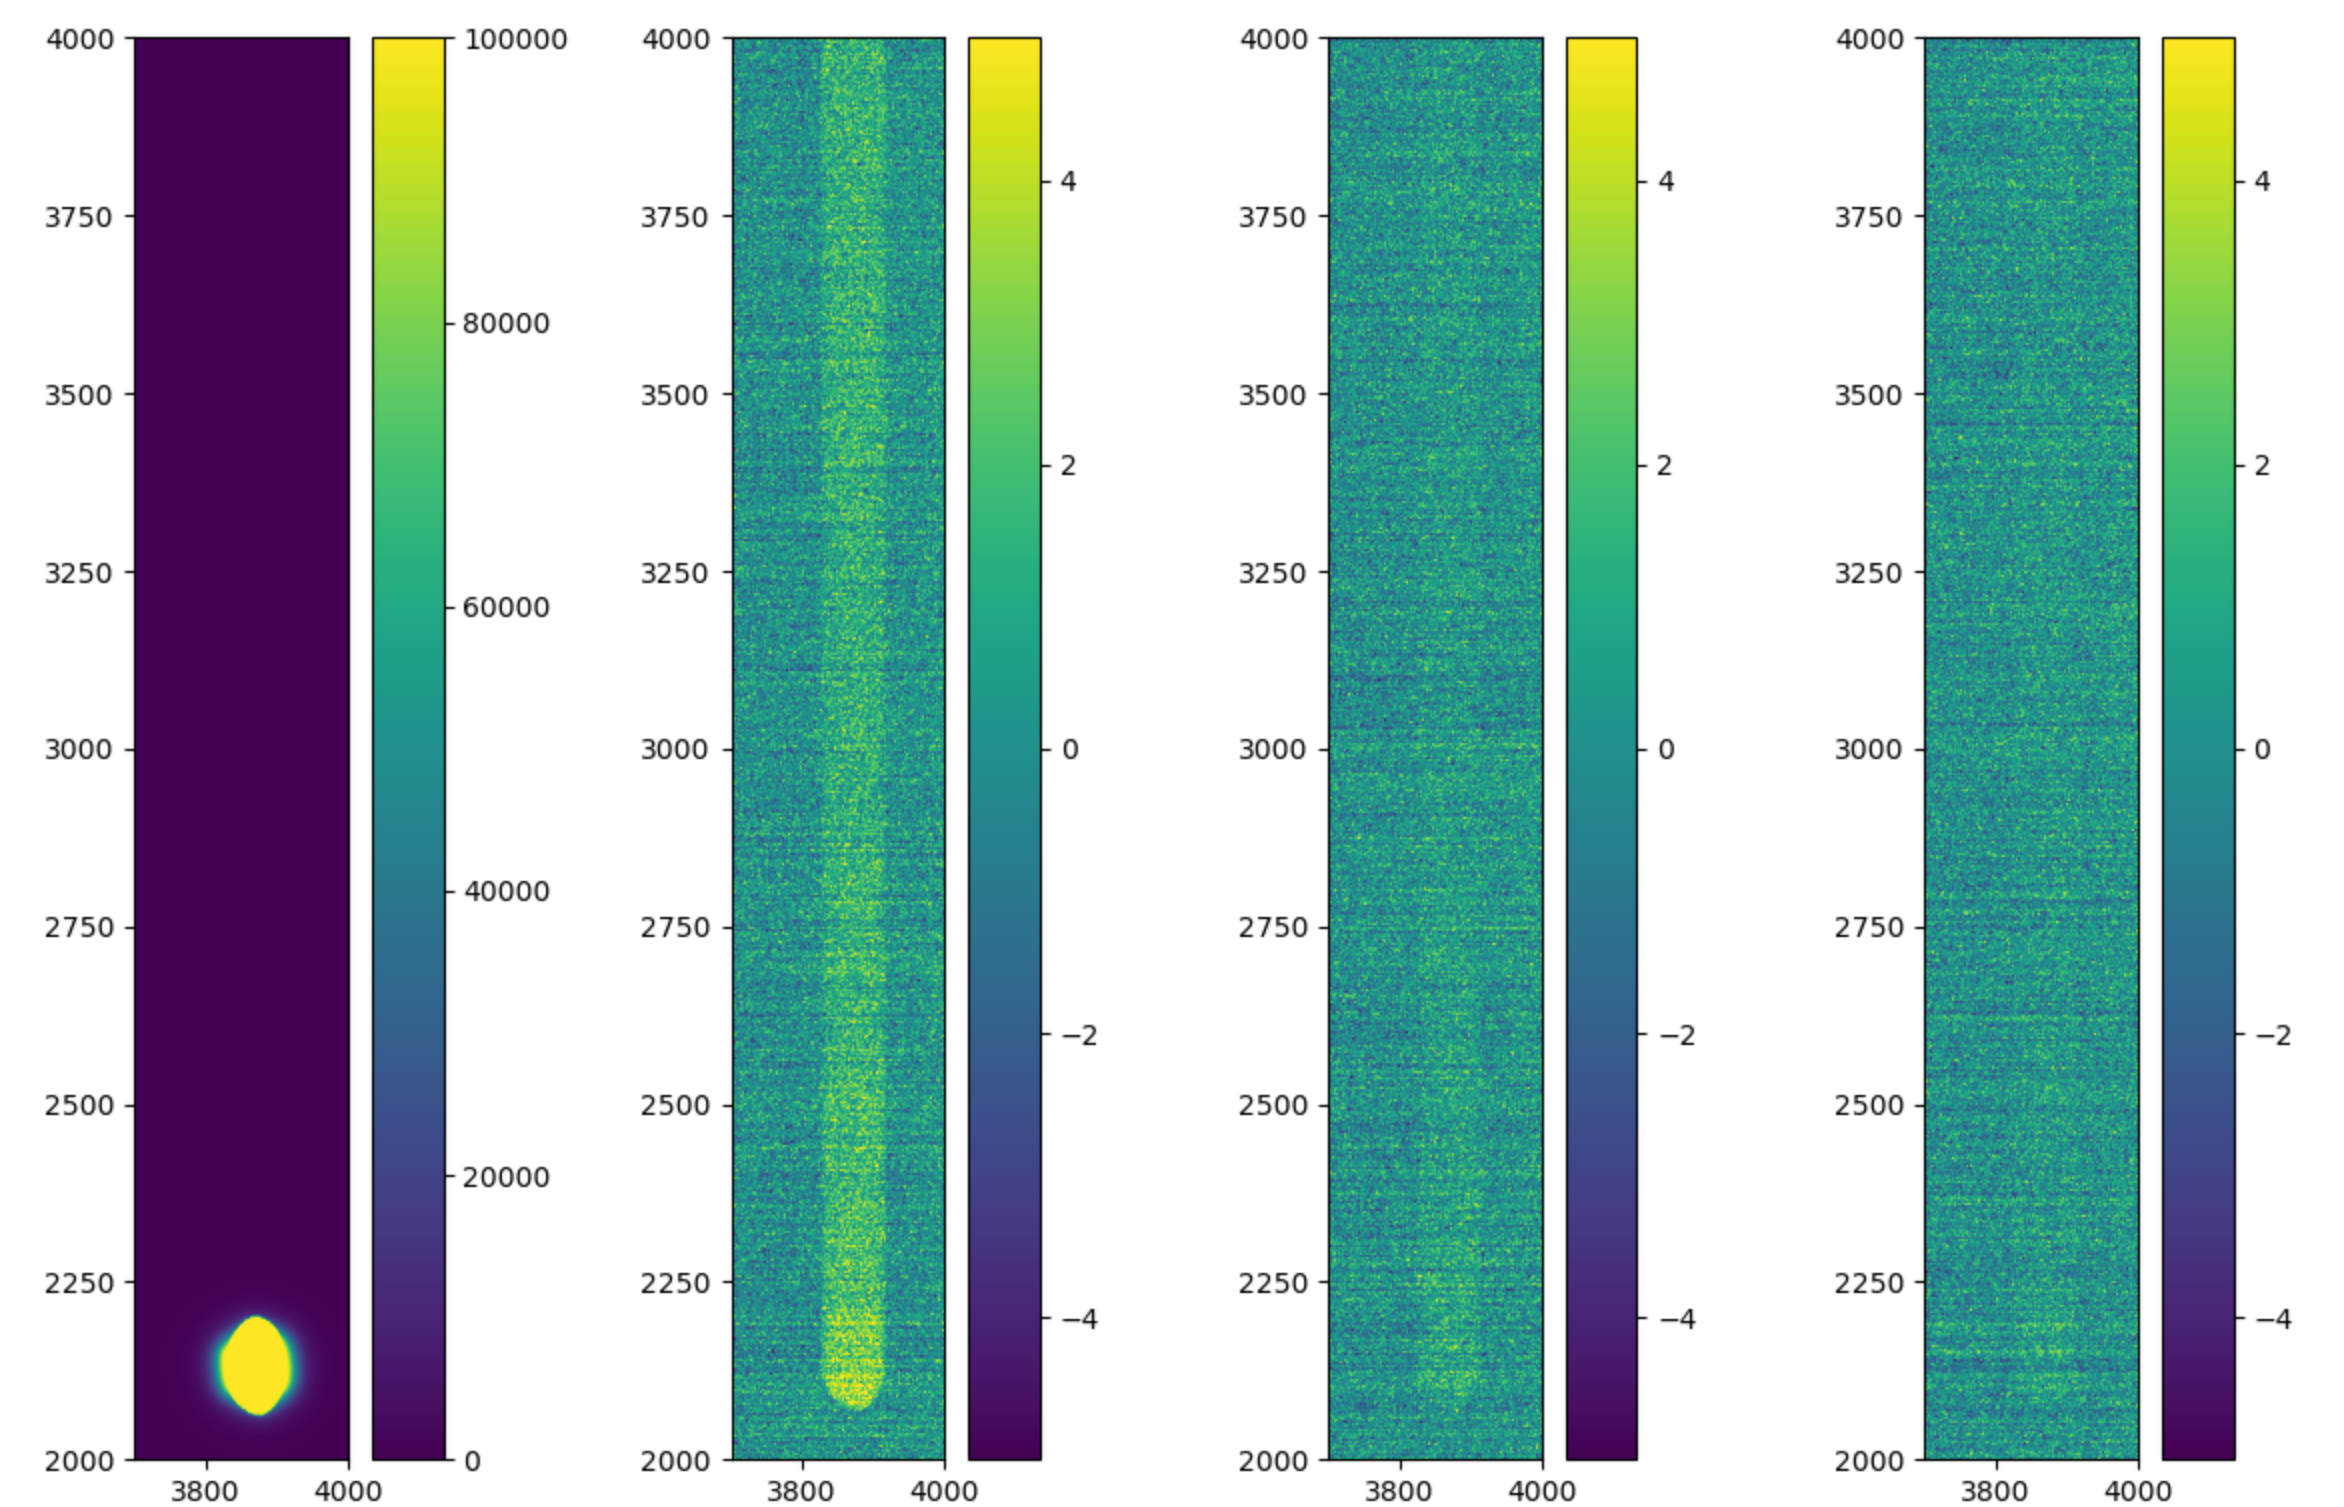
\includegraphics[width=0.95\textwidth, angle=0]{Run6_ex.png}
  \caption{
  Similar to Figure \ref{fig:ex_persistence_Run5} but with the pinhole filter. 
  This shows the initail flash and the spot (left) and the dark imgaes that followed.
  }\label{fig:Run6_example}
\end{figure*}


Using these images, we are able to measure the persistence induced by the saturated pixels as well as the trail that follows.
We then model the persistence decay using this function:
\begin{equation*}
  Counts= A * \exp(t/\tau)+c
\end{equation*}
where \textit{Coutns} are the average number of counts at the location of the spot in the following dark image, \textit{t} is the integration time since the flash, \textit{\tau} is the decay constant and \textit{A} and \textit{c} are constants.
Figure \ref{fig:Run6_decay} shows an example of the decay of the both the spot and the trail and the corresponding model fit for one detector.

\begin{figure*}[!htp]
  \centering
  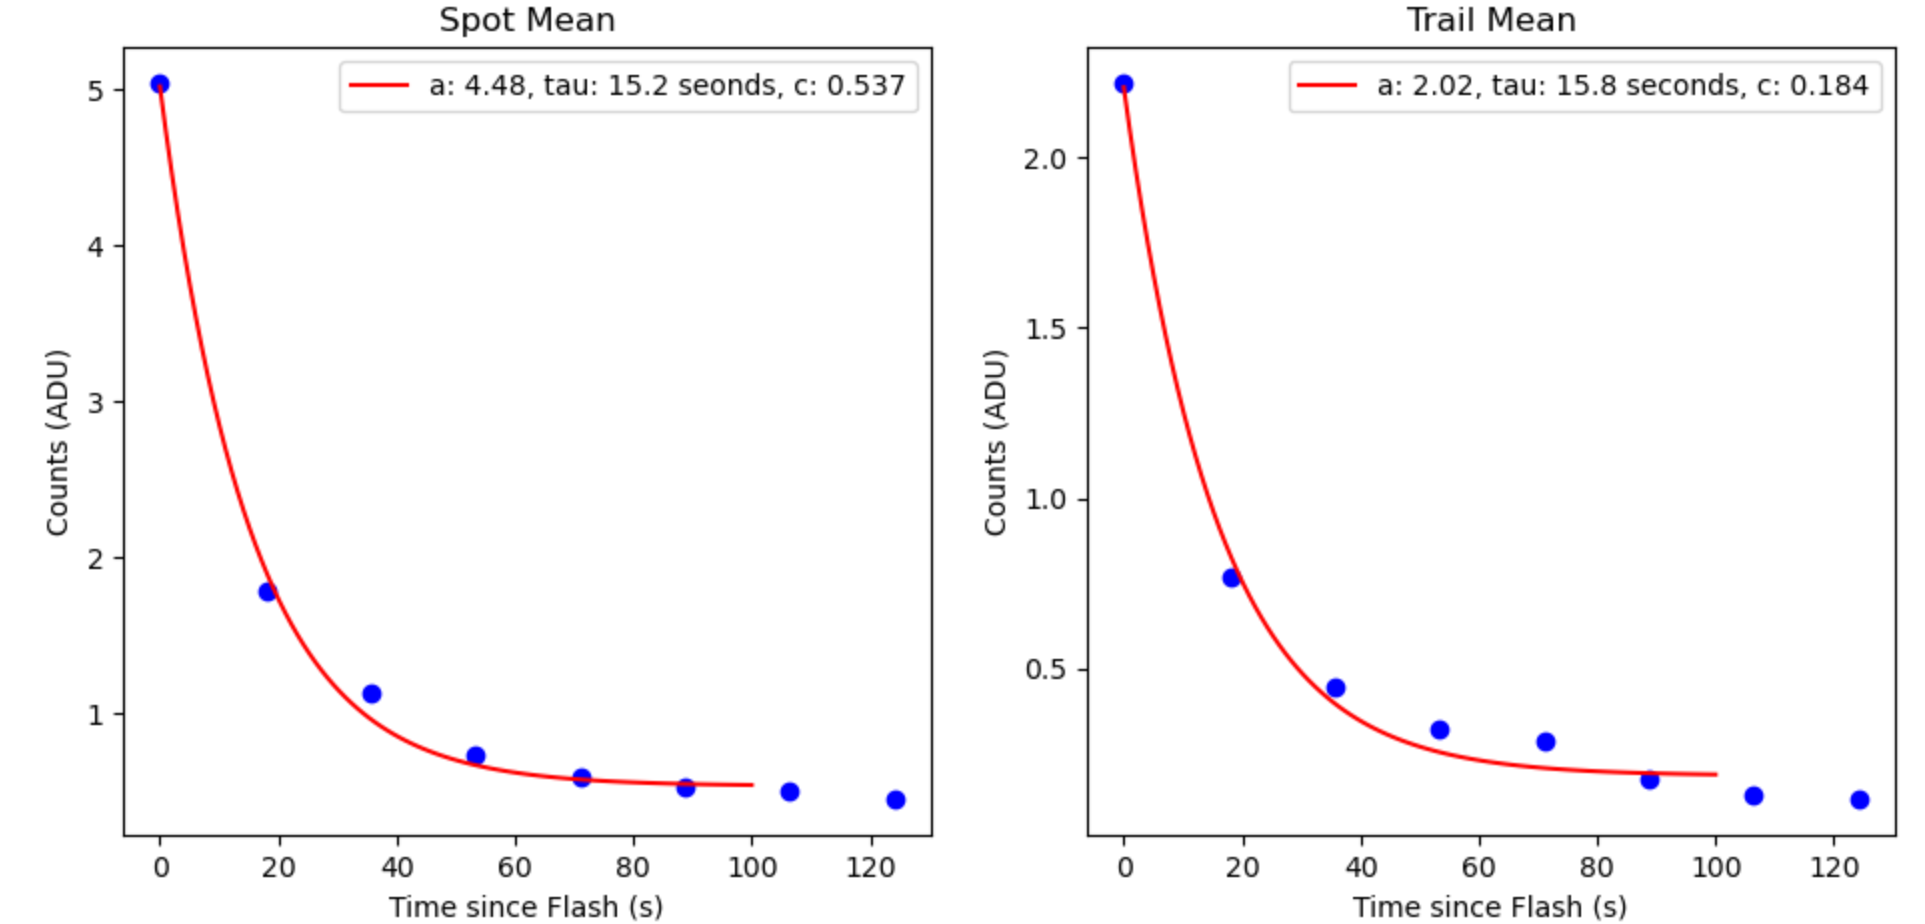
\includegraphics[width=0.95\textwidth, angle=0]{Run_6_decay.png}
  \caption{
  The decay of the persistence with consecutive dark images. 
  The blue points are the measured average counts of the spot (left) and trail (right).
  The red line shows the model fit with the parameters shown in the upper right.
  }\label{fig:Run6_decay}
\end{figure*}

Figure \ref{fig:Pers_Flash_Tau} shows the values for \textit{A} and \textit{\tau} for all detectors and all exposures that showed persistence. 
This figure shows that while \textit{\tau} is roughly the same for all images (between 10--20 seconds), the amplitude of the effect changes.
This figures points to there being a relationship between flashtime/the brightest of the spot and the persistence measured signal.

\begin{figure*}[!htp]
  \centering
  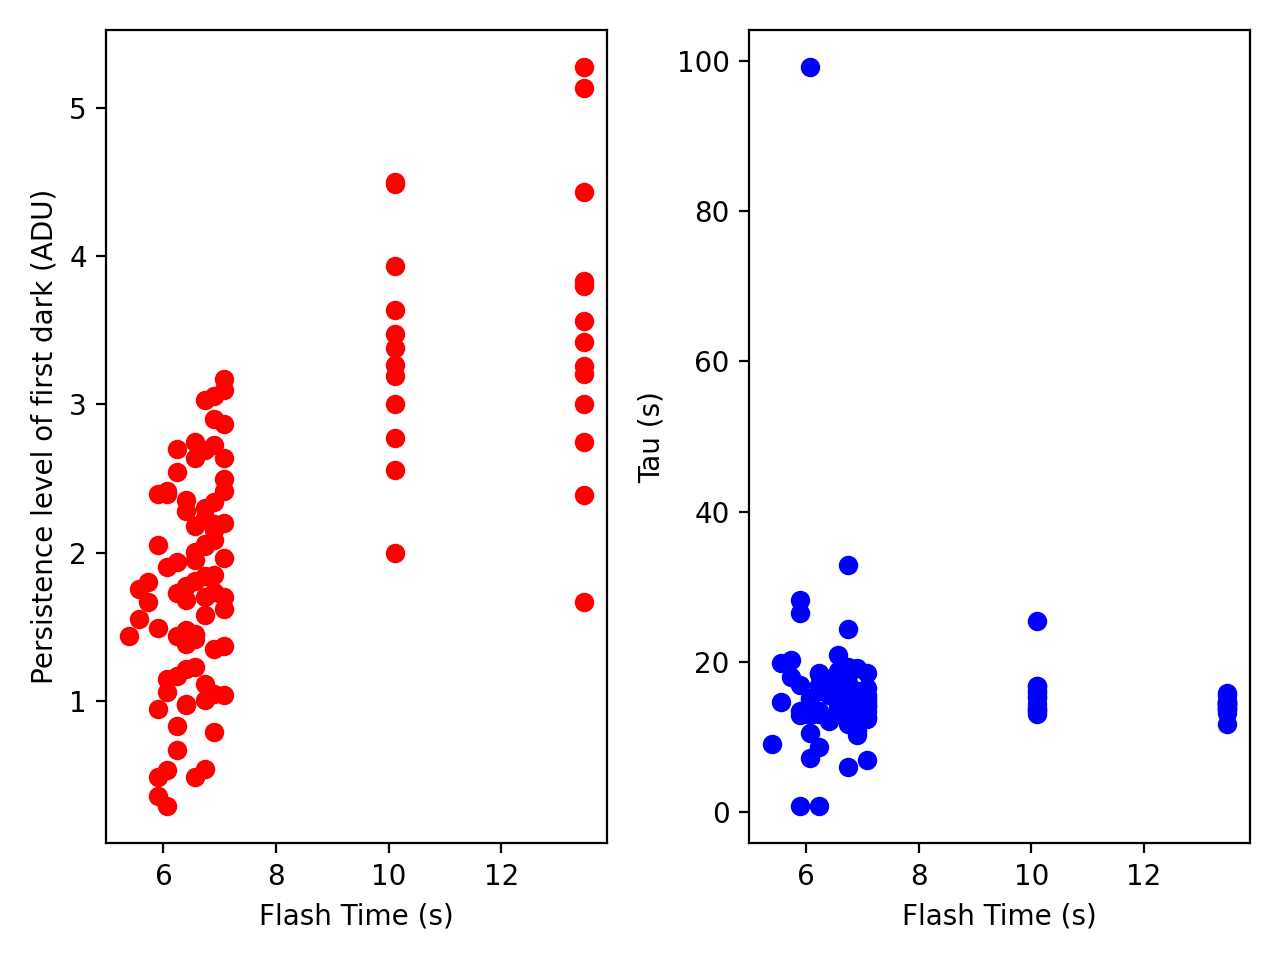
\includegraphics[width=0.95\textwidth, angle=0]{Persistence_Flash_Tau.png}
  \caption{
  The relationship between flash time (a proxy for a bright source) and amplitude (left) and tau (right) for the spot. 
  The amplitude appears to be dependent on the flash time, while tau is invariant and is consistently between 10--20 seconds. 
  }\label{fig:Pers_Flash_Tau}
\end{figure*}

\section{Effect of Persistence on DC2 Images}

Though studies are currently being done to minimize or elminate persistence, one of the next steps is to see how much persistence will affect LSST given its current rought characterization.
To study these effects, we used LSST DC2 data and the rough characterization that all persistence has a \textit{\tau} of 15 seconds and all saturated pixels have a amplitude of 5 ADU\@.
These numbers are similar to what we see with the pinhole data, which we feel will represent what on-sky data would look like better.
As most of the characterization has been with the spot and not the trail, we use 5 different schema to determine the impact of the trail: assume the trail carries with it 100\%, 75\%, 50\%, 25\%, and 0\% of the spot persistence level.
We only used one of the e2V detectors at random (detector number 88/R21-S21) for this analysis and then assume that this detector is representative of the other e2V detectors.
We also only utilize single visit images to mimic what the effect would be as images would be coming from the observatory.

\subsection{Persistence Affected Pixels}

One of the first studies we did was to look at the number of affected pixels due to persistence during a simulated night of observing.
To do this, we utilized the DC2 dataset located at the Google data facility.
Taking 4000 images, we simulated the persistence by having a running list of footprints with persistence.
If the persisence dropped below 1 ADU, the footprints were taken off the list, as this is starting to reach the level of the detector noise.
Table YYYY shows the average number of affected pixels in each of the schema.

% \begin{table}
  
% \end{table}



\subsection{Persistence Affected Objects}

Another possible metric that could be impacted by the persistence are the object measurements.
For this study, we created a new dataset type called \texttt{raw_modified}. 
This dataset type takes the \texttt{raw} file and adds the persistence model as described above utilizing the previous images.
For this study, we utilized a small subset of the DC2 dataset (68 images) and the latest reprocessing using the latest verison of the Data Release Pipeline (DRP).
We then run the \texttt{raw_modified} images through the \texttt{isr}, \texttt{characterizeImage}, and \texttt{calibrate} steps of the DRP\@. 

Figure XXX shows an example image comparing the two \textit{calexp} images from \textit{raw} and \textit{raw_modified}.

% \begin{figure*}[!htp]
%   \centering
%   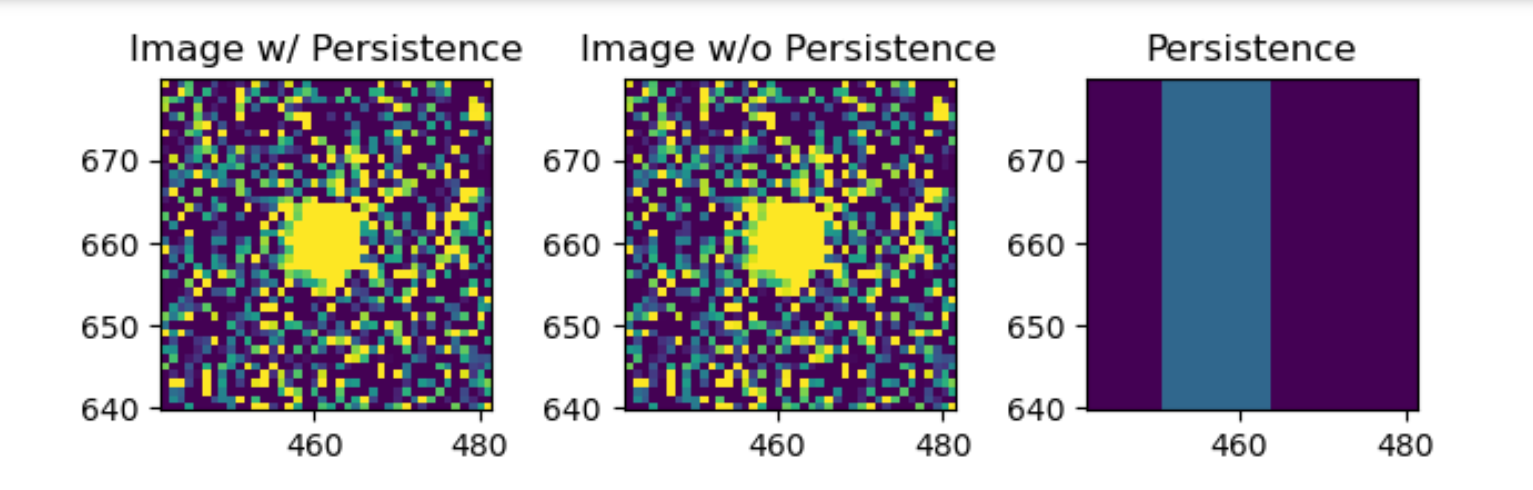
\includegraphics[width=0.95\textwidth, angle=0]{Obj_pers.png}
%   \caption{
%   A zoomed in object that shows the persistence affected image (left), the original image (middle) 
%   and the subtraction between the two to highlight the persistence (right).
%   }\label{fig:ex_persistence}
% \end{figure*}

% \begin{figure*}[!htp]
%   \centering
%   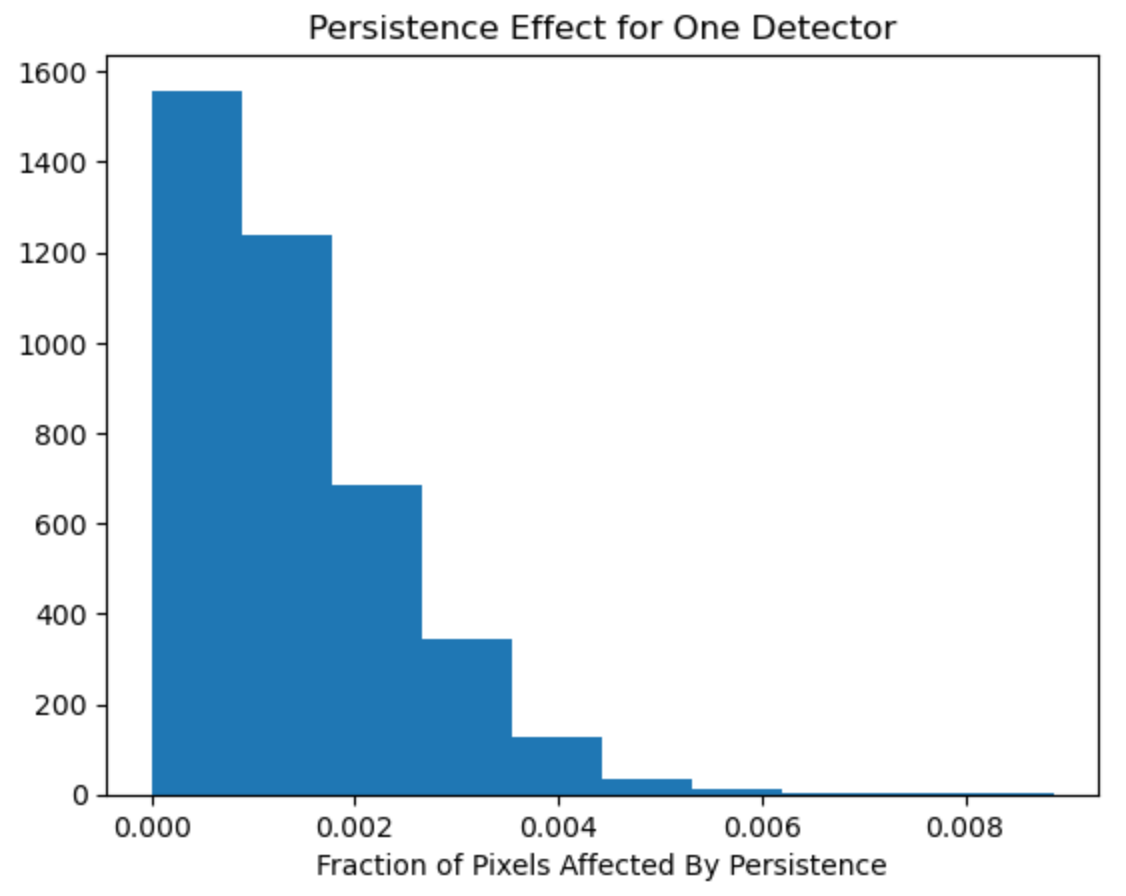
\includegraphics[width=0.95\textwidth, angle=0]{DC2_percent_affected_pixels.png}
%   \caption{
%   The percentage of affected pixels using 4000 sequential DC2 images. The majority of the images have $<0.2\%$ of their pixels affected. 
%   }\label{fig:affected_pixels}
% \end{figure*}


% Since this effect will not be easily removed, I looked into how persistence will affect LSST like images and measurements on the objects. 
% I adopted the same model as desribed above for the persistence and its trail and added it into subsquent images. 
% Figure ~\ref{fig:ex_persistence} shows an example of a DC2 image and the model persistence applied to it. 
% I then plotted a histogram of the fraction of persistence affected pixels as seen in Figure ~\ref{fig:affected_pixels}. 
% This shows the number of images with the corresponidng fraction of affected pixels. 
% For most images, $<0.2\%$ of pixels are affected in the subsquent images.


% \section{Effect of Persistence on DC2 Objects}

% \begin{figure*}[!htp]
%   \centering
%   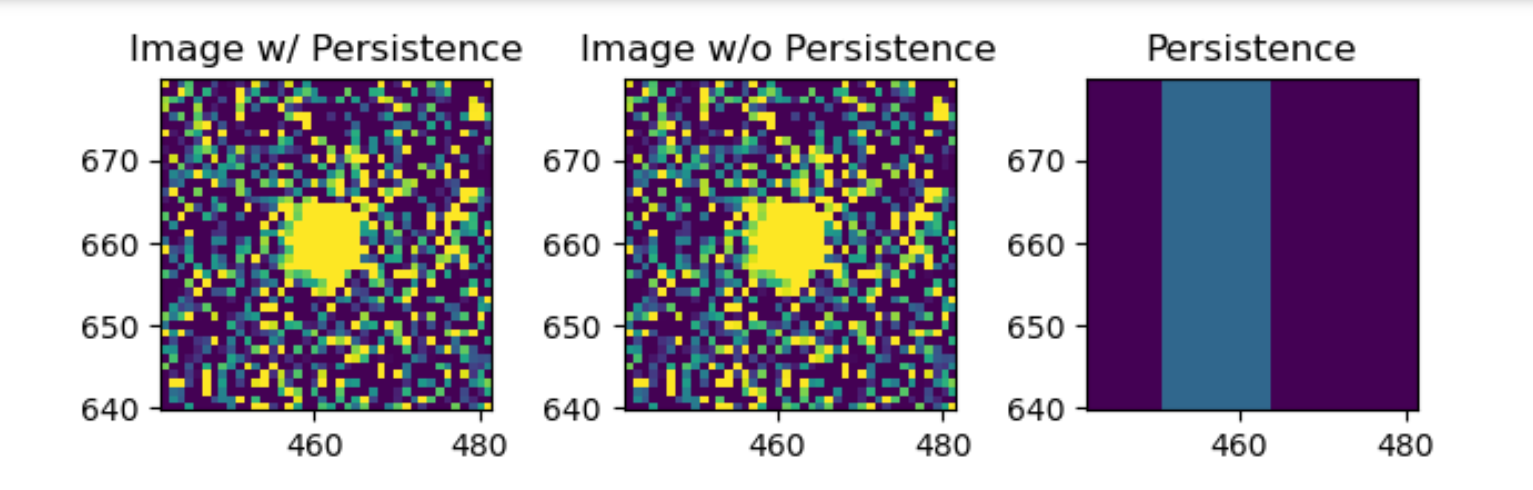
\includegraphics[width=0.95\textwidth, angle=0]{Obj_pers.png}
%   \caption{
%   A zoomed in object that shows the persistence affected image (left), the original image (middle) 
%   and the subtraction between the two to highlight the persistencet (right)
%   }\label{fig:obj_persistence}
% \end{figure*}

% To measure the effect that this would have on DC2 objects, I used a small subset of data (around 20 images) from DC2 
% found in this collection \texttt{$`2.2i/runs/test-med-1/w_2023_17/DM-39092'$}. 
% Taking the raw images from this dataset, 
% I ran a similar process to the procedure in measuring the effect on an a suite of DC2 images and added the persistence in. 
% I then saved these images as \texttt{$`raw_modified'$} images and ran these types of images through the DRP pipeline up until the `calexp' image step.
% These images can be found in the collection \texttt{$`u/banovetz/dc2/w_2023_34/raw_persistence_single_value_output'$}

% There were roughly 200 objects in these 20 images that were affected by persistence an example of which can be seen in Figure \ref{fig:obj_persistence}.
% Comparing these objects with and without persistence, 
% I found that those with persistence would have a difference of magnitude of about 0.001-0.01 magnitude for those dimmer than ~19-20 magnitude. 
% Figure \ref{fig:absolute_fractional_flux} shows the fractional magnitude difference between the persistence affected images and the originals
%  as a function of magnitude ordered objects (with 0 being the brightest object).

% \begin{figure*}[!htp]
%   \centering
%   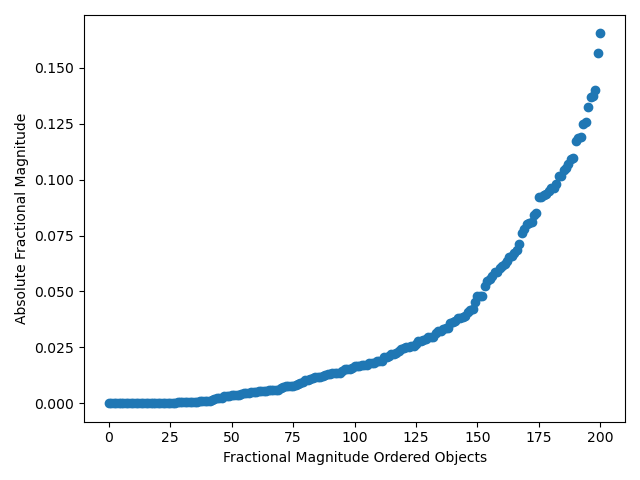
\includegraphics[width=0.95\textwidth, angle=0]{Absolute_Fractional_Magnitude.png}
%   \caption{
%   A zoomed in object that shows the persistence affected image (left), the original image (middle) 
%   and the subtraction between the two to highlight the persistencet (right)
%   }\label{fig:absolute_fractional_flux}
% \end{figure*}

% This can be explained as these objects have an area of roughtly 100 square pixels and the trails caused by the persisence can be 10--20 pixels wide.
% Increase the flux by 100--600 ADU of an object would cause this discrepancy.


\appendix

Here are the relevant collections for what we used for the DC2 comparison:


% Include all the relevant bib files.
% https://lsst-texmf.lsst.io/lsstdoc.html#bibliographies
% \section{References}\label{sec:bib}
% \renewcommand{\refname}{} % Suppress default Bibliography section
% \bibliography{local,lsst,lsst-dm,refs_ads,refs,books}

% Make sure lsst-texmf/bin/generateAcronyms.py is in your path
% \section{Acronyms}\label{sec:acronyms}
% \addtocounter{table}{-1}
\begin{longtable}{p{0.145\textwidth}p{0.8\textwidth}}\hline
\textbf{Acronym} & \textbf{Description}  \\\hline

DM & Data Management \\\hline
\end{longtable}

% If you want glossary uncomment below -- comment out the two lines above
%\printglossaries





\end{document}
